\chapter{LV 5 am 23.05.2014}
\section{Besprechung Hausaufgabe - Anforderungen}
\subsection{Funktionale Anforderungen}
\begin{itemize}
\item Ergebnis $x \in R$ : $ax^2 + bx + c = 0$
\item kein Absturz bei komplexer Lösung
\item vernünftige Reaktion auf Eingabefehler
	\begin{itemize}
		\item $a = 0$
		\item unvollständige Eingaben
		\item $4ac > b^2$
	\end{itemize}
\item relativer max. Rundungsfehler von 0,1\% mit Beweis (für die wirkliche  Realisierung darf die Formel nicht 1 zu 1 programmiert werden; in der Realität wird eher eine Newton-Annäherung implementiert).
\item es gibt immer ein definiertes Ergebnis (Ausnahmebehandlungen)
\item keine Endlosschleife (wenn Newton angewendet wird, dann braucht es eine vernünftige Abbruchbedingung)
\item Zeitbedarf max. 1 msec
	\begin{itemize}
		\item Rechner/Prozessor
		\item max. 2x SQRT der Standardimplementierung
	\end{itemize}
\item Signatur: Name, Parameter, Ergebnistyp
\end{itemize}

Jetzt soll jeder seine Lösung anhand dieser Anforderungen bewerten. Die Lösung darf auch dahingehend verbessert werden, dass alle Anforderungen erfüllt werden.

\section{Referenz-Architekturen}
Refernez-Architekturen beschreiben eine Definition typischer Strukturen. Diese sind nicht unbedingt für die Implementierung geeignet.

\begin{itemize}
\item ISO-OSI-Referenzmodell
\item ECMA-Toaster (für CASE-Umgebungen)
\item Schichtenarchitektur 
\end{itemize}

\section{Verteilte Systeme}
Die Motivation hinter verteilten Systemen ist vor allem eine bessere Ressourcenteilung. Hier sind Faktoren wie Offenheit, Nebenläufigkeit sowie Skalierbarkeit von enormer Bedeutung. Der Nachteil an solchen Systemen ist deren Komplexität.

Wir haben folgende Varianten für verteilte Systeme kennengelernt
\begin{itemize}
\item Mehrprozessor-Architekturen
\item Client/Server-Architekturen
\item Verteilte Objektarchitekturen
\item Peer-to-Peer-Architekturen
\item Dienstorientierte Architekturen
\end{itemize}

\section{Echtzeit-Software}
Echtzeitsysteme beschreiben ein Softwaresystem bei welchem die einwandfreie Funktionsweise auch von der Zeit zwischen dem Auftreten eines Stimulus und der Durchführung der entsprechenden Antwort abhängig ist. Hierbei wird zwischen einem weichen und einem harten Echtzeitsystem unterschieden.

\section{Bedienoberflächen}
Bei der Bedieneroberfläche sind drei wichtig Punkte zu beachten. Punkt eins ist die Anforderung, dass eine Oberfläche so aufgebaut ist, dass sie den Anforderungen entspricht. Punkt zwei ist die Gestaltung. Eine Oberfläche sollte nach den wünschen der Anwender gestaltet werden. Punkt drei ist der Entwurfsprozess. Dieser sollte in Zusammenarbeit mit dem Kunden erarbeitet und durchgeführt werden.

\section{Objekt-orientierter Entwurf}
Der Objekt orientierte Entwurf ist untergliedert in drei Phasen.
\begin{itemize}
\item Objekt-orientierte Analyse
\item Objekt-orientierter Enwurf
\item Objekt-orientierte Programmierung
\end{itemize}

\section{Entwicklung - Entwicklung kritischer Systeme}
Bei der Entwicklung kritischer Systeme, gibt es verschiedene (komplementäre) Strategien. Hierbei spielt vor allem die Erkennung von Fehlern eine große Bedeutung
\begin{itemize}
\item Fehlervermeidung
\item Fehlerentdeckung
\item Fehlertoleranz
\end{itemize}

Um Fehler zu erkennen, stehen folgende Techniken zur Verfügung:

\begin{itemize}
\item Verlässliche Softwareprozesse
\item Qualitätsmanagement
\item Formale Spezifikation
\item Statische Verifikation
\item Starke Typisierung
\item Sichere Programmierung
\item Ausnahmebehandlung
\item Geschützte Information
\end{itemize}

\subsection{Fehlervermeidung}
Die Fehlervermeidung beginnt bereits bei den Anforderungen. Diese müssen genau inspiziert werden. Auch ein Anforderungsmanagement ist notwendig, da sich Anforderungen ändern.
Ebenfalls wichtig ist, dass mindestens ein Vier-Augen-Prinzip bei der Codeimplementierung und dem Entwurf verfolgt wird. Des Weiteren gilt es Tests zu planen und zu managen. Auch welche Konfigurationen erstellt und ausgeliefert werden, muss klar sein.

\subsubsection{Sichere Programmierung}
Im Rahmen der sicheren Programmierung, sind mögliche Gefahrenquellen wie zum Beispiel Gotos, Rundungsfehler von Gleitkommazahlen, Pointer, dynamische Speicherallokierung, Parallelität, Rekursionen, Interrupts, Vererbung, Aliasing, sowie keine Überprüfung von Arraygrenzen und Konfigurationsdaten. 

\subsubsection{Ausnahmebehandlung}
Es sollten prinzipiell nur Sprachen verwendet werden, die eine vernünftige Ausnahmebehandlung bieten. Der Code wird dadurch wartbarer und Fehler lassen sich vermeiden.

\subsection{Fehlertoleranz}
Es gibt zwei Typen der Fehlererkennung
\begin{itemize}
\item vorbeugende Fehlererkennung
\item rückblickende Fehlererkennung
\end{itemize}

Ein wichtiges Hilfsmittel dafür stellt die Validierung da. Auch wichtig ist das Fehler reproduzierbar sind, sowie das ein System im Fehlerfall wiederhergestellt werden kann.  


\subsubsection{Fehlertolerante Architekturen}
Eine Variante ist die Verwendung von redundanter Hardware. Dabei ist es wichtig, dass auf jeder Hardware Software von unterschiedlichen Entwicklern laufen, um die Ergebnisse vergleichen zu können um so fehlertoleranter zu werden.

Eine andere Variante ist die Verwendung von sogenannten Wiederherstellungsblöcken.

\section{Weiterentwicklung}
\subsection{Ursachen der Wartung}
Wartung bedeutet nicht gleich Fehlerbehebung. Sie macht nur 17\% bei der Wartung aus. Circa 65\% machen Erweiterungen aus und weitere 18\% dies Softwareanpassung an z.B. neue Hardware.

\subsection{Wartungsaufwand}
Oftmals wird in der Praxis das Entwicklerteam nach dem Release auf ein neues Projekt angesetzt und ein anderes Team liest sich in die Software ein und wartet sie dann bzw. die Wartung wird an eine andere Firma übertragen. Das ist unter anderem ein Grund für hohen Wartungsaufwand. Oft spielen auch die Fähigkeiten (z.B. mangelnde Erfahrungen im Anwendungsgebiet oder der eingesetzten Technologie) der Entwickler, veraltete/fehlerhafte/nicht vorhandene Dokumentationen oder fehlendes Konfigurationsmanagement eine entscheidende Rolle.

Ebenfalls wichtige Einflussgrößen sind die Anzahl und Komplexität der Schnittstellen, die Anzahl der veränderlichen Anforderungen und die Geschäftsprozesse, in denen das System verwendet wird.

\subsection{Weiterentwicklungsprozesse}
Die hier angeführt Grafik verdeutlicht einen Prozess zur Software Weiterentwicklung. Es zeigt den Prozess von Sommerville 
\begin{figure}[hbtp]
\centering
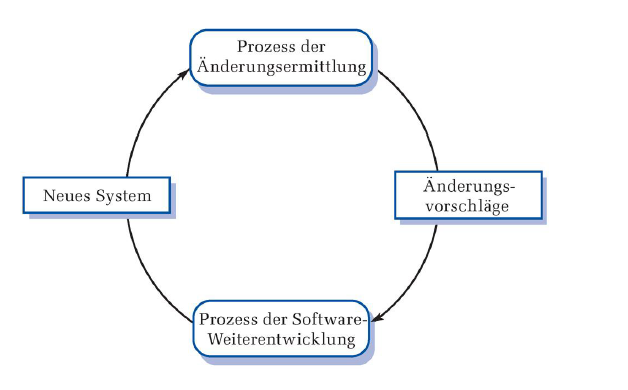
\includegraphics[scale=0.5]{document/graphics/Weiterentwicklungsprozess.png} 
\caption{Grundprozesse nach Sommerville}
\end{figure}

Bei der Weiterentwicklung ist vor allem das Ermitteln von Änderungen ein wichtiges Thema.

\begin{figure}[hbtp]
\centering
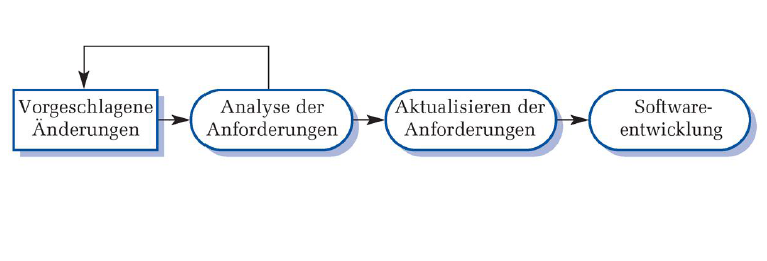
\includegraphics[scale=0.5]{document/graphics/Aenderungsermittlungsprozess.png} 
\caption{Änderungsermittlungsprozess nach Sommerville}
\end{figure}

Dabei ist zu beobachten, dass es manchmal von Nöten ist schnell Änderungen durchzuführen. Hierbei helfen natürlich gute Prozesse für die Weiterentwicklung.